% !TeX root = gbitut03.tex
%beamer

% Comment/uncomment this line to toggle handout mode
% \newcommand{\handout}{}

\ifdefined \handout
\documentclass[handout]{sdqbeamer} % Handout mode
\else
\documentclass{sdqbeamer}
\fi

%% UTF-8-Encoding
\usepackage[utf8]{inputenc}

% % \bigtimes abgeschrieben von http://tex.stackexchange.com/questions/14386/importing-a-single-symbol-from-a-different-font
% \DeclareFontFamily{U}{mathx}{\hyphenchar\font45}
% \DeclareFontShape{U}{mathx}{m}{n}{
%       <5> <6> <7> <8> <9> <10> gen * mathx
%       <10.95> mathx10 <12> <14.4> <17.28> <20.74> <24.88> mathx12
%       }{}
% \DeclareSymbolFont{mathx}{U}{mathx}{m}{n}
% \DeclareMathSymbol{\bigtimes}{\mathop}{mathx}{161}

\RequirePackage{xcolor}

\def\9{\square}
%\def\9{\blank}

% f"ur Aussagenlogik
\colorlet{alcolor}{blue}
\RequirePackage{tikz}
\usetikzlibrary{arrows.meta}
\newcommand{\alimpl}{\mathrel{\tikz[x={(0.1ex,0ex)},y={(0ex,0.1ex)},>={Classical TikZ Rightarrow[]}]{\draw[alcolor,->,line width=0.7pt,line cap=round] (0,0) -- (15,0);\path (0,-6);}}}
\newcommand{\alrimpl}{\mathrel{\tikz[x={(0.1ex,0ex)},y={(0ex,0.1ex)},>={Classical TikZ Leftarrow[]}]{\draw[alcolor,->,line width=0.7pt,line cap=round] (0,0) -- (15,0);\path (0,-6);}}}
\newcommand{\aleqv}{\mathrel{\tikz[x={(0.1ex,0ex)},y={(0ex,0.1ex)},>={Classical TikZ Rightarrow[]}]{\draw[alcolor,<->,line width=0.7pt,line cap=round] (0,0) -- (18,0);\path (0,-6);}}}
\newcommand{\aland}{\mathbin{\raisebox{-0.6pt}{\rotatebox{90}{\texttt{\color{alcolor}\char62}}}}}
\newcommand{\alor}{\mathbin{\raisebox{-0.8pt}{\rotatebox{90}{\texttt{\color{alcolor}\char60}}}}}
%\newcommand{\ali}[1]{_{\mathtt{\color{alcolor}#1}}}
\newcommand{\alv}[1]{\mathtt{\color{alcolor}#1}}
\newcommand{\alnot}{\mathop{\tikz[x={(0.1ex,0ex)},y={(0ex,0.1ex)}]{\draw[alcolor,line width=0.7pt,line cap=round,line join=round] (0,0) -- (10,0) -- (10,-4);\path (0,-8) ;}}}
\newcommand{\alvdash}{\mathrel{\tikz[x=4pt,y=3pt] {\draw[alcolor,line width=0.7pt,line cap=round,line join=round] (0,0) -- (0,1) -- (1,1) -- (0,1) -- (0,2);}}}
\newcommand{\alP}{\alv{P}} %ali{#1}}
\newcommand{\alQ}{\alv{Q}} %ali{#1}}
\newcommand{\alR}{\alv{R}} %ali{#1}}
\newcommand{\alS}{\alv{S}} %ali{#1}}
%\newcommand{\alka}{\negthinspace\hbox{\texttt{\color{alcolor}(}}}
\newcommand{\alka}{\negthinspace\text{\texttt{\color{alcolor}(}}}
%\newcommand{\alkz}{\texttt{\color{alcolor})}}\negthinspace}
\newcommand{\alkz}{\text{\texttt{\color{alcolor})}}\negthinspace}
\newcommand{\altrue}{\texttt{\textcolor{alcolor}{WAHR}}}
\newcommand{\alfalse}{\texttt{\textcolor{alcolor}{FALSCH}}}
\newcommand{\AAL}{A_{AL}}
\newcommand{\LAL}{\hbox{\textit{For}}_{AL}}
\newcommand{\AxAL}{\hbox{\textit{Ax}}_{AL}}
\newcommand{\AxEq}{\hbox{\textit{Ax}}_{Eq}}
\newcommand{\AxPL}{\hbox{\textit{Ax}}_{PL}}
\newcommand{\AALV}{\hbox{\textit{Var}}_{AL}}
\newcommand{\MP}{\hbox{\textit{MP}}}
\newcommand{\GEN}{\hbox{\textit{GEN}}}
\newcommand{\W}{\ensuremath{\hbox{\textbf{w}}}\xspace}
\newcommand{\F}{\ensuremath{\hbox{\textbf{f}}}\xspace}
\newcommand{\WF}{\ensuremath{\{\W,\F\}}\xspace}
\newcommand{\val}{\hbox{\textit{val}}}
\newcommand{\valDIb}{\val_{D,I,\beta}}

\newcommand*{\from}{\colon}

% die nachfolgenden Sachen angepasst an cmtt
\newlength{\ttquantwd}
\setlength{\ttquantwd}{1ex}
\newlength{\ttquantht}
\setlength{\ttquantht}{6.75pt}
\def\plall{%
  \tikz[line width=0.67pt,line cap=round,line join=round,baseline=(B),alcolor] {
    \draw (-0.5\ttquantwd,\ttquantht) -- node[coordinate,pos=0.4] (lll){} (-0.25pt,-0.0pt) -- (0.25pt,-0.0pt) -- node[coordinate,pos=0.6] (rrr){} (0.5\ttquantwd,\ttquantht);
    \draw (lll) -- (rrr);
    \coordinate (B) at (0,-0.35pt);
  }%
}
\def\plexist{%
  \tikz[line width=0.67pt,line cap=round,line join=round,baseline=(B),alcolor] {
    \draw (-0.9\ttquantwd,\ttquantht) -- (0,\ttquantht) -- node[coordinate,pos=0.5] (mmm){} (0,0) --  (-0.9\ttquantwd,0);
    \draw (mmm) -- ++(-0.75\ttquantwd,0);
    \coordinate (B) at (0,-0.35pt);
  }\ensuremath{\,}%
}
\let\plexists=\plexist
\newcommand{\NT}[1]{\ensuremath{\langle\mathrm{#1} \rangle}}

\newcommand{\CPL}{\text{\itshape Const}_{PL}}
\newcommand{\FPL}{\text{\itshape Fun}_{PL}}
\newcommand{\RPL}{\text{\itshape Rel}_{PL}}
\newcommand{\VPL}{\text{\itshape Var}_{PL}}
\newcommand{\ATer}{A_{\text{\itshape Ter}}}
\newcommand{\ARel}{A_{\text{\itshape Rel}}}
\newcommand{\AFor}{A_{\text{\itshape For}}}
\newcommand{\LTer}{L_{\text{\itshape Ter}}}
\newcommand{\LRel}{L_{\text{\itshape Rel}}}
\newcommand{\LFor}{L_{\text{\itshape For}}}
\newcommand{\NTer}{N_{\text{\itshape Ter}}}
\newcommand{\NRel}{N_{\text{\itshape Rel}}}
\newcommand{\NFor}{N_{\text{\itshape For}}}
\newcommand{\PTer}{P_{\text{\itshape Ter}}}
\newcommand{\PRel}{P_{\text{\itshape Rel}}}
\newcommand{\PFor}{P_{\text{\itshape For}}}

\newcommand{\plka}{\alka}
\newcommand{\plkz}{\alkz}
%\newcommand{\plka}{\plfoo{(}}
%\newcommand{\plkz}{\plfoo{)}}
\newcommand{\plcomma}{\hbox{\texttt{\color{alcolor},}}}
\newcommand{\pleq}{{\color{alcolor}\doteq}}

% MODIFIED (DJ)
% previously: \newcommand{\plfoo}[1]{\mathtt{\color{alcolor}#1}}
\newcommand{\plfoo}[1]{\texttt{\color{alcolor}#1}}

\newcommand{\plc}{\plfoo{c}}
\newcommand{\pld}{\plfoo{d}}
\newcommand{\plf}{\plfoo{f}}
\newcommand{\plg}{\plfoo{g}}
\newcommand{\plh}{\plfoo{h}}
\newcommand{\plx}{\plfoo{x}}
\newcommand{\ply}{\plfoo{y}}
\newcommand{\plz}{\plfoo{z}}
\newcommand{\plR}{\plfoo{R}}
\newcommand{\plS}{\plfoo{S}}

\newcommand{\bv}{\mathrm{bv}}
\newcommand{\fv}{\mathrm{fv}}

%\newcommand{\AxAL}{\hbox{\textit{Ax}}_{AL}}
%\newcommand{\AALV}{\hbox{\textit{Var}}_{AL}}

%\renewcommand{\#}[1]{\literal{#1}}
\newcommand{\A}{\mathcal{A}}
\newcommand{\Adr}{\text{Adr}}
\newcommand{\ar}{\mathrm{ar}}
\newcommand{\ascii}[1]{\literal{\char#1}}
%\newcommand{\assert}[1]{\text{/\!\!/\ } #1}
\newcommand{\assert}[1]{\colorbox{black!7!white}{\ensuremath{\{\;#1\;\}}}}
\newcommand{\Assert}[1]{$\langle$\textit{#1}$\rangle$}
\newcommand{\B}{\mathcal{B}}
\newcommand{\bfmod}{\mathbin{\kw{ mod }}}
\newcommand{\bb}{{\text{bb}}}
\def\bottom{\hbox{\small$\pmb{\bot}$}}
\newcommand{\card}[1]{|#1|}
%\newcommand{\cod}{\mathop{\text{cod}}}  % ist in thwmathabbrevs
\newcommand{\Conf}{\mathcal{C}}
\newcommand{\define}[1]{\emph{#1}}
%\renewcommand{\dh}{d.\,h.\@\xspace}
%\newcommand{\Dh}{D.\,h.\@\xspace}
%\newcommand{\engl}[1]{engl.\xspace\emph{#1}}
\newcommand{\eps}{\varepsilon}
%\newcommand{\evtl}{evtl.\@\xspace}
\newcommand{\fbin}{\text{bin}}
\newcommand{\finv}{\text{inv}}
\newcommand{\fnum}{\text{num}}
\newcommand{\fNum}{{\text{Num}}}
\newcommand{\frepr}{\text{repr}}
\newcommand{\fRepr}{\text{Repr}}
\newcommand{\fZkpl}{\text{Zkpl}}
\newcommand{\fLen}{\text{Len}}
\newcommand{\fsem}{\text{sem}}
\providecommand{\fspace}{\mathord{\text{space}}}
\providecommand{\fSpace}{\mathord{\text{Space}}}
\providecommand{\ftime}{\mathord{\text{time}}}
\providecommand{\fTime}{\mathord{\text{Time}}}
\newcommand{\fTrans}{\text{Trans}}
\newcommand{\fVal}{\text{Val}}

% MODIFIED (DJ)
\newcommand{\Val}{\text{Val}}

%\def\G{\mathbb{Z}}
\newcommand{\HT}[1]{\normalfont\textsc{HT-#1}}
\newcommand{\htr}[3]{\{#1\}\;#2\; \{#3\}}
\newcommand{\Id}{\text{I}}
%\newcommand{\ie}{i.\,e.\@\xspace}
\newcommand{\instr}[2]{\texttt{#1}\ \textit{#2}}
\newcommand{\Instr}[2]{\texttt{#1}\ \textrm{#2}}
\newcommand{\instrr}[3]{\texttt{#1}\ \textit{#2}\texttt{(#3)}}
\newcommand{\Instrr}[3]{\texttt{#1}\ \textrm{#2}\texttt{(#3)}}

% MODIFIED (DJ)
% previously:  \newcommand{\io}{\!\mid\!}
\newcommand{\io}{\ensuremath{\!\mid\!}}

%\usepackage{KITcolors}
\newcommand{\literal}[1]{\hbox{\textcolor{blue!95!white}{\textup{\texttt{\scalebox{1.11}{#1}}}}}}
%\newcommand{\literal}[1]{\hbox{\textcolor{KITblue!80!black}{\textup{\texttt{#1}}}}}
\def\kasten#1{\leavevmode\literal{\setlength{\fboxsep}{1pt}\fbox{\vrule  width 0pt height 1.5ex depth 0.5ex #1}}}
\newcommand{\kw}[1]{\ensuremath{\mathbf{#1}}}
\newcommand{\lang}[1]{\ensuremath{\langle#1\rangle}}
%\newcommand{\maw}{m.\,a.\,w.\@\xspace}
%\newcommand{\MaW}{M.\,a.\,w.\@\xspace}
\newcommand{\mdefine}[2][FOOBAR]{\define{#2}\def\foobar{FOOBAR}\def\optarg{#1}\ifx\foobar\optarg\def\optarg{#2}\fi\graffito{\optarg}}
\newcommand{\meins}{\rotatebox[origin=c]{180}{1}}
\newcommand{\Mem}{\text{Mem}}
\newcommand{\memread}{\text{memread}}
\newcommand{\memwrite}{\text{memwrite}}
\providecommand{\meta}[1]{\ensuremath{\langle}\textit{#1}\ensuremath{\rangle}}
%\newcommand{\N}{\mathbb{N}}
\newcommand{\NP}{\mathbf{NP}}
\newcommand{\Nadd}{N_{\text{add}}}
\newcommand{\Nmult}{N_{\text{mult}}}
% MODIFIED (DJ): added \!, mathcal{O}
\newcommand{\Oh}[1]{\mathcal{O}\!\left(#1\right)}
\newcommand{\Om}[1]{\Omega\!\left(#1\right)}
\newcommand{\personname}[1]{\textsc{#1}}
\newcommand{\regname}[1]{\texttt{#1}}
\newcommand{\mima}{\textsc{Mima}\xspace}
\newcommand{\mimax}{\textsc{Mima-X}\xspace}

\def\Pclass{\text{\bfseries P}}
\def\PSPACE{\text{\bfseries PSPACE}}

\newcommand{\SPush}{\text{push}}
\newcommand{\SPop}{\text{pop}}
\newcommand{\SPeek}{\text{peek}}
\newcommand{\STop}{\text{top}}
\newcommand{\STos}{\text{\itshape tos}}
\newcommand{\SBos}{\text{\itshape bos}}

%\newcommand{\R}{\mathbb{R}}
\newcommand{\Rnullplus}{\R_0^{+}}
\newcommand{\Rplus}{\R_{+}}
\newcommand{\resp}{resp.\@\xspace}
\newcommand{\Sem}{\text{Sem}}
\newcommand{\sgn}{\mathop{\text{sgn}}}
\newcommand{\sqbox}{\mathop{\raisebox{-6.2pt}{\hbox{\hbox to 0pt{$^{^{\sqcap}}$\hss}$^{^{\sqcup}}$}}}}
\newcommand{\sqleq}{\sqsubseteq}
\newcommand{\sqgeq}{\sqsupseteq}
% MODIFIED (DJ): added \!
\newcommand{\Th}[1]{\Theta\!\left(#1\right)}
%\newcommand{\usw}{usw.\@\xspace}
\newcommand{\V}[1]{\hbox{\textit{#1}}}
\newcommand{\x}{\times}
\newcommand{\ZK}{\mathbb{K}}
%\newcommand{\Z}{\mathbb{Z}}
\newcommand{\zB}{z.\,B.\@\xspace}
\newcommand{\ZB}{Z.\,B.\@\xspace}
% \newcommand{\bb}{{\text{bb}}}
% \def\##1{\hbox{\textcolor{darkblue}{\texttt{#1}}}}
% \def\A{\mathcal{A}}
% \newcommand{\0}{\#0}
% \newcommand{\1}{\#1}
% \newcommand{\Obj}{\text{Obj}}
% \newcommand{\start}{\mathop{\text{start}}}
% \newcommand{\compactlist}{\addtolength{\itemsep}{-\parskip}}
% \newcommand{\fval}{\text{val}}
% \newcommand{\lang}[1]{\ensuremath{\langle#1\rangle}}
% \newcommand{\io}{\!\mid\!}
% \def\sqbox{\mathop{\raisebox{-6.2pt}{\hbox{\hbox to 0pt{$^{^{\sqcap}}$\hss}$^{^{\sqcup}}$}}}}
% \def\sqleq{\sqsubseteq}
% \def\sqgeq{\sqsupseteq}
\def\Td{T_{\overline{d}}}
% \newcommand{\csym}[1]{\ensuremath{\#{c}_{\#{\hbox{\scriptsize #1}}}}}
% \newcommand{\F}{\ensuremath{\mathcal{F}}}
% \newcommand{\fsym}[2]{\ensuremath{\#{f}^{\#{\hbox{\scriptsize #1}}}_{\#{\hbox{\scriptsize #2}}}}}
% \newcommand{\rsym}[2]{\ensuremath{\#{R}^{\#{\hbox{\scriptsize #1}}}_{\#{\hbox{\scriptsize #2}}}}}
% \newcommand{\xsym}[1]{\ensuremath{\#{x}_{\#{\hbox{\scriptsize #1}}}}}
% \newcommand{\I}{\mathcal{I}}
% ********************************************************************
\usepackage{environ}
\usepackage{bm}
\usepackage{calc}
\usepackage{varwidth}
\usepackage{wasysym}
\usepackage{mathtools}


% Das ist der KIT-Stil
%\usepackage{../TutTexbib/beamerthemekit}
\titleimage{banner_2020_kit}
%\usetheme[deutsch,titlepage0]{KIT}

% Include PDFs
\usepackage{pdfpages}

% Libertine font (Original GBI font)
%\usepackage{libertine}
%\renewcommand*\familydefault{\sfdefault}  %% Only if the base font of the document is to be sans serif

% Nicer math symbols
\usepackage{eulervm}
%\usepackage{mathpazo}
\renewcommand\ttdefault{cmtt} % Computer Modern typewriter font, see lecture slides.

\usepackage{csquotes}

%%%%%%

%% Schönere Schriften
\usepackage[TS1,T1]{fontenc}

%% Bibliothek für Graphiken
\usepackage{graphicx}

%% der wird sowieso in jeder Datei gesetzt
\graphicspath{{../figures/}}

%% Anzeigetiefe für Inhaltsverzeichnis: 1 Stufe
\setcounter{tocdepth}{1}

%% Hyperlinks
\usepackage{hyperref}
% I don't know why, but this works and only includes sections and NOT subsections in the pdf-bookmarks.
\hypersetup{bookmarksdepth=subsection} 

%\usepackage{lmodern}
\usepackage{colortbl}
\usepackage[absolute,overlay]{textpos}
\usepackage{listings}
\usepackage{forloop}
%\usepackage{algorithmic} % PseudoCode package 

\usepackage{tikz}
\usetikzlibrary{matrix}
\usetikzlibrary{arrows.meta}
\usetikzlibrary{automata}
\usetikzlibrary{tikzmark}
\usetikzlibrary{positioning}

% Why has no-one come up with this yet? I mean, seriously. -.-
\tikzstyle{loop below right} = [loop, out=-60,in=-30, looseness=7]
\tikzstyle{loop below left} = [loop, out=-150,in=-120, looseness=7]
\tikzstyle{loop above right} = [loop, out=60,in=30, looseness=7]
\tikzstyle{loop above left} = [loop, out=150,in=120, looseness=7]
\tikzstyle{loop right below} = [loop below right]
\tikzstyle{loop left below} = [loop below left]
\tikzstyle{loop right above} = [loop above right]
\tikzstyle{loop left above} = [loop above left]

% Needed for gbi-macros
\usepackage{xspace}

%%%%%%

%% Verbatim
\usepackage{moreverb}

%%%%%%%%%%%%%%%%%%%%%%%%%%%%%%%%%%%% Copy end

%% Tabellen
\usepackage{array}
\usepackage{multicol}
\usepackage{hhline}

%% Bibliotheken für viele mathematische Symbole
\usepackage{amsmath, amsfonts, amssymb}

%% Deutsche Silbentrennung und Beschriftungen
\usepackage[ngerman]{babel}

%\usepackage{kbordermatrix}

% kbordermatrix settings
%\renewcommand{\kbldelim}{(} % Left delimiter
%\renewcommand{\kbrdelim}{)} % Right delimiter


% This is a configuration file with personal tutor information.
% It is therefore excluded from the git repository, so changes in this file will not conflict in git commits.

% Copy this template, rename to config.tex and add your information below.

\newcommand{\myname}{Lennart Rak}
\newcommand{\mymail}{lennart.rak@student.kit.edu} % Consider using your named student mail address to keep your u**** account private.
\newcommand{\mytutnumber}{02}

% Don't forget to update ILIAS url. WARNING: Underscores '_' and Ampersands '&' have to be escaped with backslashes '\'. Blame TeX, not me.
\newcommand{\myILIASurl}{http://s.kit.edu/gbi}

% Uncommenting this will print Socrative info with here defined roomname whenever \Socrative is called.
% (Otherwise, \Socrative will remain silent.)
% \newcommand{\mysocrativeroom}{???}

%\def\ThassesTut{}
\def\DanielsTut{}

\newcommand{\aboutMeFrame}{
	\begin{frame}{Über mich}
		\myname \\
		Informatik, 5. Fachsemester (Bachelor)
		
		% Lebensgeschichte...
		% Stammbaum...
		% Aufarbeitung der eigenen Todesser-Vergangenheit...
	\end{frame}
}
\newcommand{\aboutYouFrame}{
	\begin{frame}{Über euch}
	Wie heißt ihr? \\
	In welcher O-Phasen Gruppe wart ihr und was war euer Highlight? \\
	Habt ihr schon einen Partner zum Übungsblatt abgeben?
	    
	\end{frame}
}

\def\thisyear{2022}

% Update date of exam
\def\myKlausurtermin{27.~Februar~2023, 11:00–13:00~Uhr}

\def\mydate#1{
		  \ifnum#1=1\relax	  31. Oktober \thisyear \
	\else \ifnum#1=2\relax	  07. November \thisyear \
	\else \ifnum#1=3\relax    14. November \thisyear \
	\else \ifnum#1=4\relax    21. November \thisyear \
	\else \ifnum#1=5\relax    28. November \thisyear \
	\else \ifnum#1=6\relax    05. Dezember \thisyear \
	\else \ifnum#1=7\relax    12. Dezember \thisyear \
	\else \ifnum#1=8\relax    19. Dezember \thisyear \
	\else \ifnum#1=9\relax    09. Januar \thisyear \
	\else \ifnum#1=10\relax   16. Januar \nextyear \
	\else \ifnum#1=11\relax   23. Januar \nextyear \
	\else \ifnum#1=12\relax   30. Januar \nextyear \
	\else \ifnum#1=13\relax   06. Februar \nextyear \
	\else \ifnum#1=14\relax   13. Februar \nextyear \
	\else \textbf{Datum undefiniert!} 
	\fi\fi\fi\fi\fi\fi\fi\fi\fi\fi\fi\fi\fi\fi
}
\def\myshortdate#1{
		  \ifnum#1=1\relax	  31. 10 \thisyear \
	\else \ifnum#1=2\relax	  07. 11 \thisyear \
	\else \ifnum#1=3\relax    14. 11 \thisyear \
	\else \ifnum#1=4\relax    21. 11 \thisyear \
	\else \ifnum#1=5\relax    28. 11 \thisyear \
	\else \ifnum#1=6\relax    05. 12 \thisyear \
	\else \ifnum#1=7\relax    12. 12 \thisyear \
	\else \ifnum#1=8\relax    19. 12 \thisyear \
	\else \ifnum#1=9\relax    09. 01 \thisyear \
	\else \ifnum#1=10\relax   16. 01 \nextyear \
	\else \ifnum#1=11\relax   23. 01 \nextyear \
	\else \ifnum#1=12\relax   30. 01 \nextyear \
	\else \ifnum#1=13\relax   06. 02 \nextyear \
	\else \ifnum#1=14\relax   13. 02 \nextyear \
	\else \textbf{Datum undefiniert!} 
	\fi\fi\fi\fi\fi\fi\fi\fi\fi\fi\fi\fi\fi\fi
}

\def\mylasttimestext{Was bisher geschah...}

\colorlet{beamerlightred}{red!40}
\colorlet{beamerlightgreen}{green!50}
\colorlet{beamerlightyellow}{yellow!50}
\colorlet{lightred}{red!30}
\colorlet{lightgreen}{green!40}
\colorlet{lightyellow}{yellow!50}
\colorlet{fullred}{red!60}
\colorlet{fullgreen}{green}

\definecolor{myalertcolor}{rgb}{1,0.33,0.24}
\setbeamercolor{alerted text}{fg=myalertcolor}

% Flag to toggle display of KIT Logo.
% If you want to conform to the official logo guidelines, 
% you are not allowed to use the logo and should disable it
% using the following flag. Just saying.
% (But it's too beautiful, so best leave this commented. :P)
\newcommand{\noKITLogo}{}

% Toggle handout mode by including the following line before including PraeambelTut
% and removing the % at the start (but do NOT remove the % char here, otherwise handout mode will always be on!)
% Please keep handout mode off in all commits!

% \newcommand{\handout}{}



% define custom \handout command flag if handout mode is toggled  #DirtyAsHellButWell...
\only<beamer:0>{\def\handout{}} %beamer:0 == handout mode

\newcommand{\R}{\mathbb{R}}
\newcommand{\N}{\mathbb{N}}
\newcommand{\Z}{\mathbb{Z}}
\newcommand{\Q}{\mathbb{Q}}
\newcommand{\BB}{\mathbb{B}}
\newcommand{\C}{\mathbb{C}}
\newcommand{\K}{\mathbb{K}}
\newcommand{\G}{\mathbb{G}}
\newcommand{\nullel}{\mathcal{O}}
\newcommand{\einsel}{\mathds{1}}
\newcommand{\Pot}{\mathcal{P}}
\renewcommand{\O}{\text{O}}

\def\word#1{\hbox{\textcolor{blue}{\texttt{#1}}}}
\let\literal\word
\def\mword#1{\hbox{\textcolor{blue}{$\mathtt{#1}$}}}  % math word
\def\sp{\scalebox{1}[.5]{\textvisiblespace}}
\def\wordsp{\word{\sp}}

%\newcommand{\literal}[1]{\textcolor{blue}{\texttt{#1}}}
\newcommand{\realTilde}{\textasciitilde \ }
\newcommand{\setsize}[1]{\ensuremath{\left\lvert #1 \right\rvert}}
\newcommand{\size}[1]{\setsize{#1}}  % Shame on you, TeXStudio...
\newcommand{\set}[1]{\left\{#1\right\}}
\newcommand{\tuple}[1]{\left(#1\right)}
\newcommand{\normalvar}[1]{\text{$#1$}}

% Modified by DJ
\let\oldemptyset\emptyset
\let\emptyset\varnothing % proper emptyset

\newcommand{\boder}{\ensuremath{\mathbin{\textcolor{blue}{\vee}}}\xspace}
\newcommand{\bund}{\ensuremath{\mathbin{\textcolor{blue}{\wedge}}}\xspace}
\newcommand{\bimp}{\ensuremath{\mathrel{\textcolor{blue}{\to}}}\xspace}
\newcommand{\bgdw}{\ensuremath{\mathrel{\textcolor{blue}{\leftrightarrow}}}\xspace}
\newcommand{\bnot}{\ensuremath{\textcolor{blue}{\neg}}\xspace}
\newcommand{\bone}{\ensuremath{\textcolor{blue}{1}}\text{}}
\newcommand{\bzero}{\ensuremath{\textcolor{blue}{0}}\text{}}
\newcommand{\bleftBr}{\ensuremath{\textcolor{blue}{\texttt{(}}}\text{}}
\newcommand{\brightBr}{\ensuremath{\textcolor{blue}{\texttt{)}}}\text{}}

% Fix of \b... commands:

\renewcommand{\boder}{\alor}
\renewcommand{\bund}{\aland}
\renewcommand{\bimp}{\alimpl}
\renewcommand{\bgdw}{\aleqv}
\renewcommand{\bnot}{\alnot}
\renewcommand{\bleftBr}{\alka}
\renewcommand{\brightBr}{\alkz}
\newcommand{\alA}{\word A}
\newcommand{\alB}{\word B}
\newcommand{\alC}{\word C}

\newcommand{\plB}{\plfoo{B}}
\newcommand{\plE}{\plfoo{E}}

\newcommand{\summe}[2]{\sum\limits_{#1}^{#2}}
\newcommand{\limes}[1]{\lim\limits_{#1}}

%\newcommand{\numpp}{\advance \value{weeknum} by -2 \theweeknum \advance \value{weeknum} by 2}
%\newcommand{\nump}{\advance \value{weeknum} by -1 \theweeknum \advance \value{weeknum} by 1}

\newcommand{\mycomment}[1]{}
\newcommand{\Comment}[1]{}

%% DISCLAIMER START 
% It is INSANELY IMPORTANT NOT TO DO THIS OUTSIDE BEAMER CLASS! IN ARTCILE DOCUMENTS, THIS IS VERY LIKELY TO BUG AROUND!
\makeatletter%
\@ifclassloaded{beamer}%
{
	% TODO 
	% no time... later.   (= never -.-)
	% redefine section to ignore multiple \section calls with the same title
}%
{
	\errmessage{ERROR: section command redefinition outside of beamer class document! Please contact the author of this code or read the F-ing disclaimer.}
}%
\makeatother%
%% DISCLAIMER END

\newcounter{abc}
\newenvironment{alist}{
  \begin{list}{(\alph{abc})}{
      \usecounter{abc}\setlength{\leftmargin}{8mm}\setlength{\labelsep}{2mm}
    }
}{\end{list}}


\newcommand{\stdarraystretch}{1.20}
\renewcommand{\arraystretch}{\stdarraystretch}  % for proper row spacing in tables

\newcommand{\morescalingdelimiters}{   % for proper \left( \right) typography
	\delimitershortfall=-1pt  
	\delimiterfactor=1
}

\newcommand{\centered}[1]{\vspace{-\baselineskip}\begin{center}#1\end{center}\vspace{-\baselineskip}}

% for \implitem and \item[bla] stuff to look right:
\setbeamercolor*{itemize item}{fg=black}
\setbeamercolor*{itemize subitem}{fg=black}
\setbeamercolor*{itemize subsubitem}{fg=black}

\setbeamercolor*{description item}{fg=black}
\setbeamercolor*{description subitem}{fg=black}
\setbeamercolor*{description subsubitem}{fg=black}

\renewcommand{\qedsymbol}{\textcolor{black}{\openbox}}

\renewcommand{\mod}{\mathop{\textbf{mod}}}
\renewcommand{\div}{\mathop{\textbf{div}}}

\newcommand{\ceil}[1]{\left\lceil#1\right\rceil}
\newcommand{\floor}[1]{\left\lfloor#1\right\rfloor}
\newcommand{\abs}[1]{\left\lvert #1 \right\rvert}
\newcommand{\Matrix}[1]{\begin{pmatrix} #1 \end{pmatrix}}
\newcommand{\braced}[1]{\left\lbrace #1 \right\rbrace}

% "something" placeholder. Useful for repairing spacing of operator sections, like `\sth = 42`.
\def\sth{\vphantom{.}}

\def\fract#1/#2 {\frac{#1}{#2}} % ! Trailing space is crucial!
\def\dfract#1/#2 {\dfrac{#1}{#2}} % ! Trailing space is crucial!

\newcommand{\Mid}{\;\middle|\;}

\let\after\circ



\def\·{\cdot}
\def\*{\cdot}
\def\?>{\ensuremath{\rightsquigarrow}}  % Fuck you, Latex
\def\~~>{\ensuremath{\rightsquigarrow}}  

\newcommand{\tight}[1]{{\renewcommand{\arraystretch}{0.76} #1}}
\newcommand{\stackedtight}[1]{\renewcommand{\arraystretch}{0.76} \begin{matrix} #1 \end{matrix} }
\newcommand{\stacked}[1]{\begin{matrix} #1 \end{matrix} }
\newcommand{\casesl}[1]{\delimitershortfall=0pt  \left\lbrace\hspace{-.3\baselineskip}\begin{array}{ll} #1 \end{array}\right.}
\newcommand{\casesr}[1]{\delimitershortfall=0pt  \left.\begin{array}{ll} #1 \end{array}\hspace{-.3\baselineskip}\right\rbrace}
\newcommand{\caseslr}[1]{\delimitershortfall=0pt  \left\lbrace\hspace{-.3\baselineskip}\begin{array}{ll} #1 \end{array}\hspace{-.3\baselineskip}\right\rbrace}

\def\q#1uad{\ifnum#1=0\relax\else\quad\q{\the\numexpr#1-1\relax}uad\fi}
% e.g. \q1uad = \quad, \q2uad = \qquad etc.

\newcommand{\qqquad}{\q3uad}
\newcommand{\minusquad}{\hspace{-1em}}

%% Placeholder utils
% \§{#1}   Saves #1 as placeholder and prints it
% \.       Prints an \hphantom with the size of the recalled placeholder.
\def\indentstring{}
\def\§#1{\def\indentstring{#1}#1}
\def\.{{$\hphantom{\text{\indentstring}}$}}
%% Placeholder utils end

\newcommand{\impl}{\ifmmode\ensuremath{\mskip\thinmuskip\Rightarrow\mskip\thinmuskip}\else$\Rightarrow$\fi\xspace}
\newcommand{\Impl}{\ifmmode\implies\else$\Longrightarrow$\fi\xspace}

\newcommand{\derives}{\Rightarrow}

\newcommand{\gdw}{\ifmmode\mskip\thickmuskip\Leftrightarrow\mskip\thickmuskip\else$\Leftrightarrow$\fi\xspace}
\newcommand{\Gdw}{\ifmmode\iff\else$\Longleftrightarrow$\fi\xspace}

% Legacy code from the algo tutorial slides. Perhaps useful. Try with care.
\mycomment{
	\newcommand{\impl}{\ifmmode\ensuremath{\mskip\thinmuskip\Rightarrow\mskip\thinmuskip}\else$\Rightarrow$\xspace\fi}  
	\newcommand{\Impl}{\ifmmode\implies\else$\Longrightarrow$\xspace\fi}
	
	\newcommand{\gdw}{\ifmmode\mskip\thickmuskip\Leftrightarrow\mskip\thickmuskip\else$\Leftrightarrow$\xspace\fi}
	\newcommand{\Gdw}{\ifmmode\iff\else$\Longleftrightarrow$\xspace\fi}
}
	
\newcommand{\gdwdef}{\ifmmode\mskip\thickmuskip:\Leftrightarrow\mskip\thickmuskip\else:$\Leftrightarrow$\xspace\fi}
\newcommand{\Gdwdef}{\ifmmode\mskip\thickmuskip:\Longleftrightarrow\mskip\thickmuskip\else:$\Longleftrightarrow$\xspace\fi}

\newcommand{\symbitemnegoffset}{\hspace{-.5\baselineskip}}
\newcommand{\implitem}{\item[\impl\symbitemnegoffset]}
\newcommand{\Implitem}{\item[\Impl\symbitemnegoffset]}


\newcommand{\forcenewline}{\mbox{}\\}

\newcommand{\bfalert}[1]{\textbf{\alert{#1}}}
\let\elem\in   % I'm a Haskell freak. Don't judge me. :P


\def\|#1|{\text{\normalfont #1}}  % | steht für senkrecht (anstatt kursiv wie sonst im math mode)


% proper math typography
\newcommand{\functionto}{\longrightarrow}
\renewcommand{\geq}{\geqslant}
\renewcommand{\leq}{\leqslant}
\let\oldsubset\subset
\renewcommand{\subset}{\subseteq} % for all idiots out there using subset

\newenvironment{threealign}{%
	\[
	\begin{array}{r@{\ }c@{\ }l}
}{%
	\end{array}	
	\]
}

\newcommand{\concludes}{ \\ \hline  }
\newcommand{\deduction}[1]{
	\begin{varwidth}{.8\linewidth}
		\begin{tabular}{>{$}c<{$}}
			#1
		\end{tabular}
	\end{varwidth}	
}

\definecolor{hoareorange}{rgb}{1,.85,.6}
\newcommand{\hoareassert}[1]{\setlength{\fboxsep}{1pt}\setlength{\fboxrule}{-1.4pt}\fcolorbox{white}{hoareorange}{\ensuremath{\{\;#1\;\}}}\setlength\fboxrule{\defaultfboxrule}\setlength{\fboxsep}{3pt}}

\newcommand{\mailto}[1]{\href{mailto:#1}{{\textcolor{blue}{\underline{#1}}}}}
\newcommand{\urlnamed}[2]{\href{#2}{\textcolor{blue}{\underline{#1}}}}
\renewcommand{\url}[1]{\urlnamed{#1}{#1}}

\newcommand{\hanging}{\hangindent=0.7cm}
\newcommand{\indented}{\hanging}


% \hstretchto prints #2 left-aligned into a box of the width of #1
\def\hstretchto#1#2{%
	\mbox{}\vphantom{#2}\rlap{#2}\hphantom{#1}%
}

\def\vstretchto#1#2{%
	\mbox{}\hphantom{#2}\smash{#2}\vphantom{#1}%
}

% \hstretchtocentered prints #2 centered into a box of the width of #1
\def\hstretchtocentered#1#2{%
	\mbox{}\vphantom{#2}\scalebox{0.5}{\hphantom{#1}}\clap{#2}\scalebox{0.5}{\hphantom{#1}}%
}

% vertical centering
\newcommand{\vertcenter}[1]{%
	\ensuremath{\vcenter{\hbox{#1}}}%
}


%requires \thisyear to be defined (s. config.tex)!
\edef\nextyear{\the\numexpr\thisyear+1\relax}


% --- \frameheight constant ---
\newlength\fullframeheight
\newlength\framewithtitleheight
\setlength\fullframeheight{.92\textheight}
\setlength\framewithtitleheight{.86\textheight}

\newlength\frameheight
\setlength\frameheight{\fullframeheight}

\let\frametitleentry\relax
\let\oldframetitle\frametitle
\def\newframetitle#1{\global\def\frametitleentry{#1}\if\relax\frametitleentry\relax\else\setlength\frameheight{\framewithtitleheight}\fi\oldframetitle{#1}}
\let\frametitle\newframetitle

\def\newframetitleoff{\let\frametitle\oldframetitle}
\def\newframetitleon{\let\frametitle\newframetitle}
% --- \frameheight constant end ---

\newcommand{\fakeframetitle}[1]{%
	\vspace{-2.05\baselineskip}%
	{\Large \textbf{#1}} \\%
	\smallskip
}



\newenvironment{headframe}{\Huge THIS IS AN ERROR. PLEASE CONTACT THE ADMIN OF THIS TEX CODE. (headframe env def failed)}{}
\RenewEnviron{headframe}[1][]{
	\begin{frame}\frametitle{\ }
		\centering
		\Huge\textbf{\textsc{\BODY} \\
		}
		\Large {#1}
		\frametitle{\ }
	\end{frame}
}


\makeatletter
% Provides color if undefined.
\newcommand{\colorprovide}[2]{%
	\@ifundefinedcolor{#1}{\colorlet{#1}{#2}}{}}
\makeatother


\colorprovide{lightred}{red!30}
\colorprovide{lightgreen}{green!40}
\colorprovide{lightyellow}{yellow!50}
\colorprovide{lightblue}{blue!10}
\colorprovide{beamerlightred}{lightred}
\colorprovide{beamerlightgreen}{lightgreen}
\colorprovide{beamerlightyellow}{lightyellow}
\colorprovide{beamerlightblue}{lightblue}
\colorprovide{fullred}{red!60}
\colorprovide{fullgreen}{green}
\definecolor{darkred}{RGB}{115,48,38}
\definecolor{darkgreen}{RGB}{48,115,38}
\definecolor{darkyellow}{RGB}{100,100,0}

\only<handout:0>{\colorlet{adaptinglightred}{beamerlightred}}
\only<handout:0>{\colorlet{adaptinglightgreen}{beamerlightgreen}}
\only<handout:0>{\colorlet{adaptinglightyellow}{beamerlightyellow}}
\only<handout:0>{\colorlet{adaptinglightblue}{beamerlightblue}}
\only<beamer:0>{\colorlet{adaptinglightred}{lightred}}
\only<beamer:0>{\colorlet{adaptinglightgreen}{lightgreen}}
\only<beamer:0>{\colorlet{adaptinglightyellow}{lightyellow}}
\only<beamer:0>{\colorlet{adaptinglightblue}{lightblue}}
\only<handout:0>{\colorlet{adaptingred}{lightred}}
\only<beamer:0>{\colorlet{adaptingred}{fullred}}
\only<handout:0>{\colorlet{adaptinggreen}{lightgreen}}
\only<beamer:0>{\colorlet{adaptinggreen}{fullgreen}}



\newcommand{\TrueQuestion}[1]{
	\TrueQuestionE{#1}{}
}

\newcommand{\YesQuestion}[1]{
	\YesQuestionE{#1}{}
}

\newcommand{\FalseQuestion}[1]{
	\FalseQuestionE{#1}{}
}

\newcommand{\NoQuestion}[1]{
	\NoQuestionE{#1}{}
}

\newcommand{\DependsQuestion}[1]{
	\DependsQuestionE{#1}{}
}

\newcommand{\QuestionVspace}{\vspace{4pt}}
\newcommand{\QuestionParbox}[1]{\begin{varwidth}{.85\linewidth}#1\end{varwidth}}
\newcommand{\ExplanationParbox}[1]{\begin{varwidth}{.97\linewidth}#1\end{varwidth}}
\colorlet{questionlightgray}{gray!23}
\let\defaultfboxrule\fboxrule

% #1: bg color
% #2: fg color short answer
% #3: short answer text
% #4: question
% #5: explanation
\newcommand{\GenericQuestion}[5]{
	\setlength\fboxrule{2pt}
	\only<+|handout:0>{\hspace{-2pt}\fcolorbox{white}{questionlightgray}{\QuestionParbox{#4} \quad\textbf{?}}}
	\visible<+->{\hspace{-2pt}\fcolorbox{white}{#1}{\QuestionParbox{#4} \quad\textbf{\textcolor{#2}{#3}}} \if\relax#5\relax\else\ExplanationParbox{#5}\fi} \\
	\setlength\fboxrule{\defaultfboxrule}
}

% #1: Q text
% #2: Explanation
\newcommand{\TrueQuestionE}[2]{
	\GenericQuestion{adaptinglightgreen}{darkgreen}{Wahr.}{#1}{#2}
}

% #1: Q text
% #2: Explanation
\newcommand{\YesQuestionE}[2]{
	\GenericQuestion{adaptinglightgreen}{darkgreen}{Ja.}{#1}{#2}
}

% #1: Q text
% #2: Explanation
\newcommand{\FalseQuestionE}[2]{
	\GenericQuestion{adaptinglightred}{darkred}{Falsch.}{#1}{#2}
}

% #1: Q text
% #2: Explanation
\newcommand{\NoQuestionE}[2]{
	\GenericQuestion{adaptinglightred}{darkred}{Nein.}{#1}{#2}
}

% #1: Q text
% #2: Explanation
\newcommand{\DependsQuestionE}[2]{
	\GenericQuestion{adaptinglightyellow}{darkyellow}{Je nachdem!}{#1}{#2}
}

% #1: Q text
% #2: Answer
\newcommand{\ContentQuestion}[2]{
	\GenericQuestion{adaptinglightblue}{black}{\minusquad}{#1}{#2}
}

%\ifnum\thisyear=2018 \else \errmessage{Old ILIAS link inside preamble. Please update.} \fi

\newcommand{\ILIAS}{\urlnamed{ILIAS}{\myILIASurl}\xspace}
\newcommand{\Klausurtermin}{\myKlausurtermin\xspace}

\newcommand{\Socrative}{\ifdefined\mysocrativeroom \only<handout:0>{socrative.com $\quad \~~> \quad $ Student login \\ Raumname:  \mysocrativeroom\\ \medskip}\else\fi}

\newcommand{\thasse}[1]{
	\ifdefined\ThassesTut #1\xspace \else\fi
}
\newcommand{\daniel}[1]{
	\ifdefined\DanielsTut #1\xspace \else\fi
}
\newcommand{\thassedaniel}[2]{\ifdefined\ThassesTut #1\else\ifdefined\DanielsTut #2\fi\fi\xspace}

\ifdefined\ThassesTut \ifdefined\DanielsTut \errmessage{ERROR: Both ThassesTut and DanielsTut flags are set. This is most likely an error. Please check your config.tex file.} \else \fi \else \ifdefined\DanielsTut \else \errmessage{ERROR: Neither ThassesTut  nor DanielsTut flags are set. This is most likely an error. Please check your config.tex file.} \fi\fi

%\newcommand{\sgn}{\text{sgn}}

%%%%%%%%%%%% INHALT %%%%%%%%%%%%%%%%

%% Wochennummer
\newcounter{weeknum}

%% Titelinformationen
\title[GBI-Tutorium \mytutnumber, Woche \theweeknum]{Grundbegriffe der Informatik Tutorium \mytutnumber}

\subtitle{Woche \theweeknum \xspace}
\author[\myname]{\myname \xspace \normalfont (\mailto{\mymail})}
\groupname{KIT -- Karlsruher Institut für Technologie}
\date[\myshortdate{\theweeknum}]{\mydate{\theweeknum}}

% Modified, DJ (better safe than sorry)
%\AuthorTitleSep{ – }

%% Titel einfügen
\newcommand{\titleframe}{\KITtitleframe}

%% Alles starten mit \starttut{X}
\newcommand{\starttut}[1]{\setcounter{weeknum}{#1}\pdfinfo{
		/Author (\myname)
		/Title  (GBI-Tutorium \mytutnumber, Woche \theweeknum)
	}\titleframe\frame{\frametitle{Inhalt}\tableofcontents} \AtBeginSection[]{%
		\begin{frame}{Wo sind wir gerade?}
		\tableofcontents[currentsection]
	\end{frame}\addtocounter{framenumber}{-1}}}


\newcommand{\framePrevEpisode}{
\begin{headframe}
	\mylasttimestext
\end{headframe}
}

\newcommand{\lastframetitled}[6]{
% 	\frame{\frametitle{#6}
% 		\vspace{-#2\baselineskip}
% 		\begin{figure}[H]
% 			\centering
% 			\LARGE \textbf{\textsc{#5}} \\
% 			\vspace{.2\baselineskip}
% 			\includegraphics[#1]{#3}
% 			\vspace{-6pt}
% 			\begin{center}
% 				\small \url{#4} 
% 			\end{center}
% 		\end{figure} 
% 	}
\begin{frame}[plain]
    \vspace{\baselineskip}
    \centering
    \Large\textbf{#6}
    \begin{figure}[H]
		\centering
% 		\LARGE \textbf{\textsc{#5}} \\
% 		\vspace{.2\baselineskip}
		\includegraphics[#1]{#3}
		\vspace{-6pt}
		\begin{center}
			\small \url{#4} 
		\end{center}
	\end{figure}
\end{frame}
}

% #1 number
% #2 title 
% #3 vspace (positive) without unit (\baselineskip)
\newcommand{\xkcdframe}[3]{
	\lastframetitled{width=.96\textwidth}{#3}{xkcd/#1}{http://xkcd.com/#1}{}{#2}
}

\newcommand{\xkcdframevert}[3]
{
	\lastframetitled{height=.96\frameheight}{#3}{xkcd/#1}{http://xkcd.com/#1}{}{#2}
}

% #1 number
% #2 title 
% #3 vspace (positive) without unit (\baselineskip)
% #4 \includegraphics[] optional parameters
\newcommand{\xkcdframecustom}[4]
{
	\lastframetitled{#4}{#3}{xkcd/#1}{http://xkcd.com/#1}{}{#2}
}

\newcommand{\slideThanks}{
	\begin{frame}
	\frametitle{Credits}
	\begin{block}{}
		An der Erstellung des Foliensatzes haben mitgewirkt:\\[1em]
		Daniel Jungkind \\
		Thassilo Helmold \\
		Philipp Basler \\
		Nils Braun \\
		Dominik Doerner \\
		Ou Yue \\
	\end{block}
\end{frame}
}

%% Wörter DEPRECATED! DO NOT USE
\newcommand{\code}[1]{$\mathbf{#1}$}

\morescalingdelimiters

\begin{document}
\starttut{3}

\framePrevEpisode

\subsection{Wahr oder Falsch?}

\begin{frame}[t]{Wahr oder Falsch?}
	\delimitershortfall=0pt
	\FalseQuestionE{$\word{aaba} \in \{ \word a, \word b\}^2\times\{\word a,\word b\}^2$}{Aber: $(\word{aa}, \word{ba}) \in \{\word a, \word b\}^2\times\{\word a, \word b\}^2$}
	\FalseQuestionE{$\setsize{\{ \eps \}} = 0$}{$\{ \eps \} \neq \{\}$}
	\FalseQuestionE{Wenn $\eps \in A^*$, dann $\size{\eps^3} = 3$.}{$\size{\eps^3} = 0$; außerdem gilt $\eps \in A^*$  immer, also für alle Alphabete $A$.}
\end{frame}



\section{Aussagenlogik}

\thasse{ % No time this year...
	\frame{
		\frametitle{Ein bekanntes Logikrätsel}
		\vspace{-2pt}
		\begin{figure}[H]
			\centering
			\only<1|handout:1>{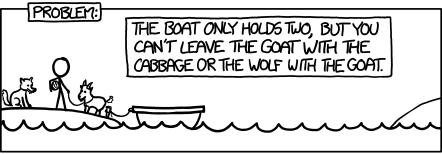
\includegraphics[scale=1]{xkcd/logic_boat_problem}}
			\only<2|handout:2>{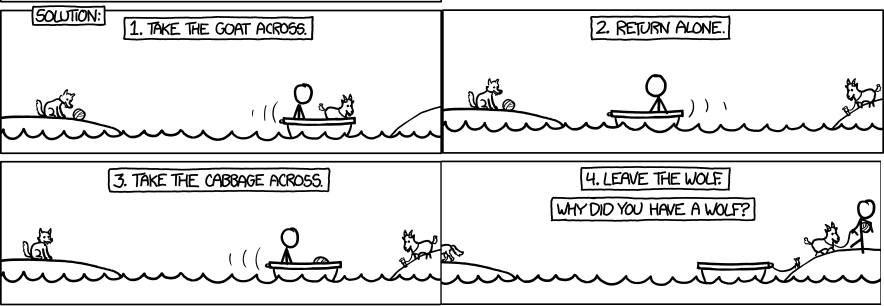
\includegraphics[scale=0.35]{xkcd/logic_boat_sol}}
			\vspace{-2pt}
			\url{http://xkcd.com/1134/}
		\end{figure} 
	}
}

\begin{frame}{Aussagenlogik}
	Aussagen sind Sätze, die entweder \textbf{wahr} oder \textbf{falsch} sind.\\
	Deren Wahrheitswert muss dabei nicht unbedingt bekannt oder \enquote{tatsächlich ermittelbar} sein.
	
	\pause
	\begin{Beispiel}
		\begin{itemize}
			\item „$ 1 + 1 = 2 $“ ist eine Aussage. Sie ist wahr.
			\item \enquote{Es gibt nur endlich viele Primzahlen.} ist eine Aussage. Sie ist falsch.
			\pause
			\item Die Goldbachsche Vermutung (Jede gerade Zahl größer 2 ist Summe zweier Primzahlen) \pause ist eine Aussage. Ihr Wahrheitswert ist unbekannt.
			\pause
			\item „Die Welt wird am 11.11.11111 untergehen.“ \pause ist auch eine Aussage. Wir werden ihren Wahrheitswert aber wohl niemals ermitteln können.
			\pause
			\item \enquote{Gelb} ist keine Aussage.
			\pause
			\item \enquote{Dieser Satz ist falsch.} \pause ist keine Aussage. Dem Satz kann offensichtlich kein Wahrheitswert zugeordnet werden.
		\end{itemize}
	\end{Beispiel}
\end{frame}

\begin{frame}{Zwei Grundsätze der Aussagenlogik}
	
	\begin{itemize}
		\pause
		\item[1.] Jede Aussage ist \textbf{entweder} wahr \textbf{oder} falsch.\\
		Wir schreiben im Folgenden $\BB= \{\W, \F\}$
		\pause
		\item[2.] Der Wahrheitswert einer \textbf{zusammengesetzten} Aussage ist durch die
		Wahrheitswerte der \textbf{Teilaussagen} eindeutig festgelegt. \\
		\enquote{$2 + 2 = 5 \; \bimp \; \text{Pinguine können fliegen}$} ist \textbf{wahr}.\\[0.2em]
		%TODO
		%Ex falso quodlibet
	\end{itemize}

	\impl Weg vom Inhalt und betrachte stattdessen \textbf{Aussagevariablen}.
\end{frame}

\begin{frame}{Syntax}
	\begin{Definition}
		$Var_{AL}$ ist die Menge aller \textbf{Aussagevariablen}. \\
		Wir bilden aussagenlogische Formeln als Wörter über dem Alphabet $A_{AL} = \{ \bleftBr, \brightBr, \bnot, \bund, \boder, \bimp \} \cup Var_{AL}$ 
	\end{Definition}
	\pause
	\begin{Definition}
		$For_{AL}$ ist die Menge aller \textbf{syntaktisch korrekten Formeln} über $Var_{AL}$.\\
		\medskip
		%(VL: induktive Definition über Konstruktionsabbildungen) \\
		Klammern, die überflüssig sind, können weg. Wir lesen es dann wie gewohnt (\enquote{$\bnot$} vor \enquote{ $\bund$} vor \enquote{ $\boder$} vor \enquote{ $\bimp$}  {\small \#PunktVorStrichUndSo}).
	\end{Definition}
\end{frame}

\begin{frame}{Syntax}
	\begin{Beispiel}
		$$Var_{AL} = \{\alA, \alB, \alC\}$$
		$$For_{AL} = \set{\alka \alA  \bimp \alB \alkz \boder \bnot \alB \bund \alC, \ \alC \bimp \alka \bnot \alC \alkz, ...}$$ 
	\end{Beispiel}
\end{frame}

\begin{frame}{Semantik}
	Die Semantik einer aussagenlogischen Formel wird durch ihre \textbf{Auswertung} bestimmt.\\
	Hierbei werden den Operatorsymbolen aus $A_{AL}$ boolesche Funktionen zugeordnet.
	
	\pause
	\begin{Definition}
		Eine \textbf{boolesche Funktion} ist eine Abbildung der Form
		$f \from \BB^n \functionto \BB$.
	\end{Definition}

	\pause
	\begin{Beispiel}
		\enquote{Handelsübliche} boolesche Funktionen sind  $b_{\bnot}$,
		$b_{\bund}$, $b_{\boder}$ und $b_{\bimp}$. 
	\end{Beispiel}
\end{frame}

\begin{frame}{Semantik}
	\let\w\W
	\let\f\F
	\begin{center}
		\begin{huge}
			$$\only<1-2|handout:1>{\bnot}\only<3-4|handout:2>{\bund}\only<5-6|handout:3>{\boder}\only<7-8|handout:4>{\bimp}$$
		\end{huge}
		Wahrheitstabelle: \\
		\medskip
		\only<1-2|handout:1>{
			\begin{tabular}{|c|c|}
				\hline 
				$A$ &  $\bnot A$ \\
				\hline
				\w & \uncover<2|handout:1>{\f} \\
				\hline
				\f & \uncover<2|handout:1>{\w} \\
				\hline
			\end{tabular}
		}
		\only<3-4|handout:2>{ 
			\begin{tabular}{|c|c|c|}
				\hline 
				$A$ & $B$ & $A \mathop{\bund} B$ \\
				\hline
				\w & \w & \uncover<4|handout:2>{\w} \\
				\hline
				\w & \f & \uncover<4|handout:2>{\f} \\
				\hline
				\f & \w & \uncover<4|handout:2>{\f} \\
				\hline
				\f & \f & \uncover<4|handout:2>{\f} \\
				\hline
			\end{tabular}
		}
		\only<5-6|handout:3>{ 
			\begin{tabular}{|c|c|c|}
				\hline 
				$A$ & $B$ & $A \mathop{\boder} B$ \\
				\hline
				\w & \w & \uncover<6|handout:3>{\w} \\
				\hline
				\w & \f & \uncover<6|handout:3>{\w} \\
				\hline
				\f & \w & \uncover<6|handout:3>{\w} \\
				\hline
				\f & \f & \uncover<6|handout:3>{\f} \\
				\hline
			\end{tabular}
		}
		\only<7-8|handout:4>{
			\begin{tabular}{|c|c|c|}
				\hline 
				$A$ & $B$ & $A \mathop{\bimp} B$ \\
				\hline
				\w & \w & \uncover<8|handout:4>{\w} \\
				\hline
				\w & \f & \uncover<8|handout:4>{\f} \\
				\hline
				\f & \w & \uncover<8|handout:4>{\w} \\
				\hline
				\f & \f & \uncover<8|handout:4>{\w} \\
				\hline
			\end{tabular}
		}
	\end{center}
\end{frame}

\begin{frame}{Semantik}
	Wenn wir den Wahrheitswert einer \textbf{zusammengesetzten} Aussage bestimmen wollen, brauchen wir die Werte der \textbf{verwendeten Aussagenvariablen}. \\
	\begin{Definition}
		Sei $V \subseteq Var_{AL}$ die Menge der verwendeten Aussagevariablen.\\
		Eine Funktion $I \from V \functionto \BB$ bezeichnet man als \textbf{Interpretation}.
	\end{Definition}
	
	

\end{frame}

\begin{frame}{Auswertung}
	\begin{Definition}
		Sei $I$ eine Interpretation. Dann liefert die Abbildung $val_I(A)$ den Wahrheitswert zu einer aussagenlogischen Formel $A$. \\
		\medskip
		Diese Funktion nennen wir \textbf{Auswertung} und berechnen sie schrittweise, z.~B.:
	\end{Definition}
	
	\begin{align*}
	&val_I(\alka\alA \bimp \alB\alkz \boder \bnot \alB)  \\
	\visible<2->{= \;&b_{\boder} (val_I(\alA\bimp \alB), val_I(\bnot \alB)) \\}
	\visible<3->{= \;&b_{\boder} (b_{\bimp} (val_I(\alA), val_I(\alB)), b_{\bnot}(val_I(\alB))) \\}
	\visible<4->{= \;&b_{\boder} (b_{\bimp} (I(\alA), I(\alB)), b_{\bnot}(I(\alB))) \\}
	\end{align*}
\end{frame}

\begin{frame}{Auswertung}
	\begin{Definition}
		Eine \textbf{Tautologie} ist eine aussagenlogische Formel, bei der für alle möglichen Interpretationen $I$ gilt: $val_I(A) = \W$. \\
		\impl Schreibweise: \quad $\models A$ \\
		\medskip
		
		\pause
		Zwei aussagenlogische Formeln $A$ und $B$ heißen \textbf{äquivalent}, wenn für jede beliebige Interpretation $I$
		$$val_I(A) = val_I(B)$$
		gilt. \\
		\impl Schreibweise: \quad $A \equiv B$
	\end{Definition}
\end{frame}

% TODO
\begin{frame}[t]{Auswertung}
	\only<all:1>{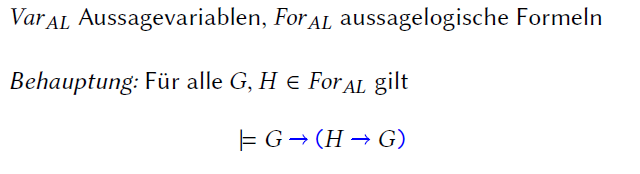
\includegraphics[scale=0.65]{aussagenlogik/al_uebung_1}\\[2em]
	Quelle: GBI-Übung 2015/2016}
	\only<all:2>{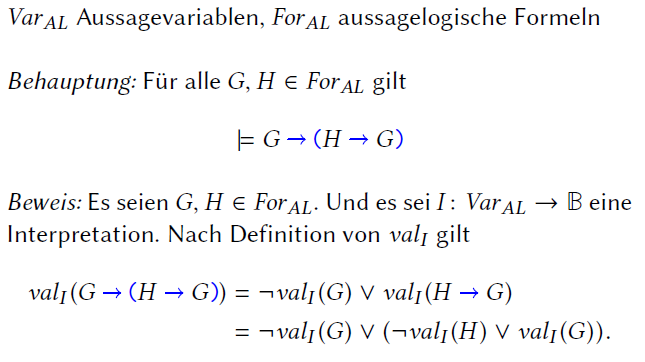
\includegraphics[scale=0.6]{aussagenlogik/al_uebung_2}}
	\only<all:3>{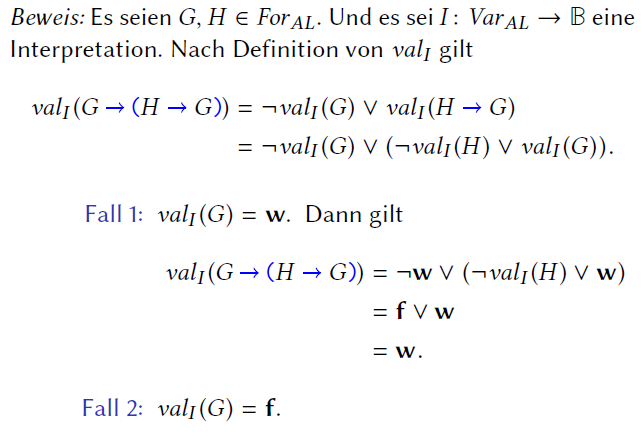
\includegraphics[scale=0.6]{aussagenlogik/al_uebung_3}}
	\only<all:4>{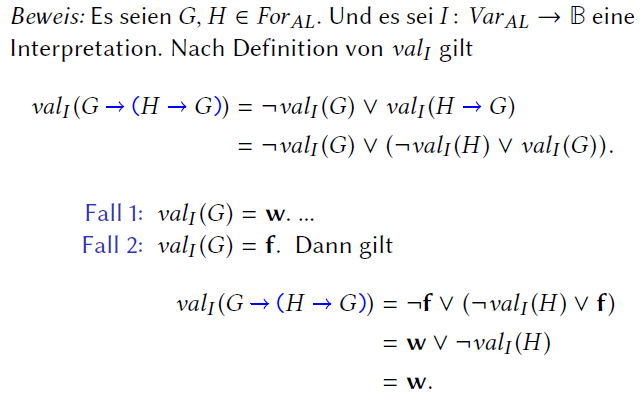
\includegraphics[scale=0.6]{aussagenlogik/al_uebung_4}}
	\only<all:5>{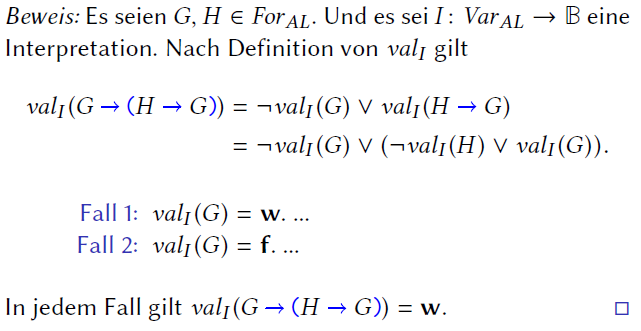
\includegraphics[scale=0.6]{aussagenlogik/al_uebung_5}}
\end{frame}

\begin{frame}{Semantik}
	
	Möchte man eine AL-Formel für alle möglichen Interpretationen auswerten, so macht man dies meist in Form einer \textbf{Wahrheitstabelle}.
	
	\begin{block}{Aufgabe}
		Gegeben seien die Formeln
		$$ F_1 = \left(\left(\left(\alB \bimp \alA \right) \boder \alB \right) \bimp (\bnot \alA)\right) \bund \alB$$
		und
		$$F_2 = \bnot \alA \bund \alB$$
		Stellt die Wahrheitstabellen von $F_1$ und $F_2$ auf. Sind die beiden Formeln äquivalent?
	\end{block}
\end{frame}

\begin{frame}{Lösung}
	Für die Formel $F_1$:
	\begin{table}[H]
	\centering
	\begin{tabular}{|*{6}{c|}}
	\hline
	$\alA$ & $\alB$ & $\alB \bimp \alA$ &  $\dots \boder \alB$ & $\dots \bimp \bnot \alA$ & $\dots \bund \alB$ \pause \\ \hline
	\W & \W & \W & \W & \F & \F  \\ \hline \pause
	\W &  \F & \W & \W & \F & \F  \\ \hline \pause
	\F & \W & \F & \W & \W & \W  \\ \hline \pause
	\F & \F & \W & \W & \W & \F \\ \hline
	\end{tabular}
	\end{table}
\end{frame}

\begin{frame}{Lösung}
	Für die Formel $F_2$:
	\begin{table}[h!]
	\centering
	\begin{tabular}{|*{3}{c|}}
	\hline
	$\alA$ & $\alB$ & $\bnot \alA \bund \alB$  \\ \hline \pause
	\W & \W & \F \\  \hline \pause
	\W & \F & \F \\  \hline \pause
	\F & \W & \W \\  \hline \pause
	\F & \F & \F \\ \hline
	\end{tabular}
	\end{table}
	Also sind die beiden Formeln äquivalent: $$F_1 \equiv F_2$$
\end{frame}


\newcommand{\alnand}{\alv{\bar \land}}

%Übungsaufgabe 3.2 WS22/23
\begin{frame}{NAND}
	Man nennt eine Menge von Konnektiven, mit denen alle boolenschen Funktonen
	als aussagenlogische Formel ausgedrückt werden können, eine Basis der Aussagenlogik.
	Das aussagenlogische Konnektiv $NAND (\alv{ \bar \land})$ ist definiert als
	\begin{align*}
		val_I (G \aland H) = 
		\begin{cases}
			\W, & \text{falls } val_I(G) = \F \text{ oder } val_I (H) = \F \\
			\F, & \text{sonst}
		\end{cases}
	\end{align*}
	für beliebige Fromeln $G, H \in \LAL$

	\visible<+(-1)>{}
	\begin{alist}
		\item Geben Sie die Wahrheitstabelle für $G \alnand H$ an.
		\item Zeigen Sie dass $\alnand$ eine Basis ist. Geben Sie dafür (ohne Beweis)
		für die folgenden Formeln je eine äquivalente aussagenlogische Formel an, die nur $\alnand$ benutzt:
		\begin{enumerate}[i]
			\item $\bnot \plfoo{P}$ 
			\visible<+-|handout:2->{
				$\equiv \plfoo{P} \alnand \plfoo{P}$
			}
			\item $\plfoo{P} \bund \plfoo{Q}$
			\visible<+-|handout:2->{
				$ \equiv \bleftBr \plfoo{P} \alnand \plfoo{Q} \brightBr \alnand \bleftBr \plfoo{P} \alnand \plfoo{Q} \brightBr$
			}
			\item $\plfoo{P} \boder \plfoo{Q}$
			\visible<+-|handout:2->{
				$ \equiv \bleftBr \plfoo{P} \alnand \plfoo{P} \brightBr \alnand \bleftBr \plfoo{Q} \alnand \plfoo{Q} \brightBr$
			}
			\item $\plfoo{P} \bimp \plfoo{Q}$
			\visible<+-|handout:2->{
				$ \equiv \plfoo{P} \alnand \bleftBr \plfoo{Q} \alnand \plfoo{Q} \brightBr$
			}
		\end{enumerate}
	\end{alist}
\end{frame}

\section{Beweisbarkeit}

\begin{frame}{Modelle}
	\begin{Definition}
		Sei $G$ eine aussagenlogische Formel. \\
		Eine Interpretation $I$ heißt \textbf{Modell} von $G$, wenn gilt: \quad $val_I(G) = \W$. \\
		\pause
		\medskip
		Sei $\Gamma$\thasse{\footnote{Gamma}} eine Formelmenge.
		Eine Interpretation $I$ heißt \textbf{Modell} von $\Gamma$, wenn für alle Formeln $G \in  \Gamma$ gilt: \quad $val_I(G) = \W$.
	\end{Definition}
	\pause
	\begin{block}{Schreibweisen}
		$\Gamma \models G$: jedes Modell von $\Gamma$ auch Modell von $G$ \\
		Beispiel: \quad $\set{A,B,C} \models G$ \quad Jedes Modell von $A, B$ \textbf{und} $C$ ist auch Modell von $G$ \\
		\medskip
		Schreibe $H \models G$ statt $\set{H} \models G$ \\
		\medskip
		Schreibe $\models G$ statt $\set{} \models G$ \\
		\impl G ist \emph{Tautologie} oder \emph{allgemeingültig} 
	\end{block}
\end{frame}

\begin{frame}{Modelle}
	\begin{Definition}
		Eine Formel $G$ heißt \textbf{erfüllbar}, wenn für mindestens ein $I$ wahr. \\
		
	\end{Definition}
	\pause
	\begin{Beispiel}
		Alle Modelle von \mword{(C \boder \bnot C) \bimp \left(\bnot(B \bimp A)\right)}? \\
		\pause
		\impl $I_1, I_2 \from \set{\word A, \word B, \word C} \functionto \BB, \; 
		I_1(v) = 
		\caseslr{\F, & v = \word A \\
				\W, & v = \word B \\
				\W, & v = \word C}, \;
		I_2(v) = 
		\caseslr{\F, & v = \word A \\
				\W, & v = \word B \\
				\F, & v = \word C}$. \\
		\impl Formel \emph{erfüllbar}. \\
		\pause
		\medskip
		Alle Modelle von \mword{\bnot(C \bimp C)}? \\
		\pause
		\impl Gibt keine, Formel \emph{unerfüllbar}.
	\end{Beispiel}
\end{frame}

\begin{frame}{Tautologie, Äquivalenz}
	\begin{Definition}
		Eine Formel $G$ heißt \textbf{Tautologie}, wenn für alle möglichen $I$ wahr. \\
		\pause
		\medskip
		Kurzschreibweise: Für Formeln $G$ und $H$ ist \\
		$$\bleftBr G \bgdw H \brightBr :\equiv \bleftBr\bleftBr G \bimp H \brightBr \bund \bleftBr H \bimp G\brightBr\brightBr$$ \\
		\medskip
		\alert{\textbf{Bitte aufpassen mit Pfeilen: \quad $\bgdw$ vs. $\gdw$ \quad $\bimp$ vs. $\impl$}}
	\end{Definition}
	\pause
	\begin{block}{Lemma}
		Für Formeln $G$ und $H$ gilt \\
		\[ G \equiv H \quad \text{ genau dann, wenn } \quad G \bgdw H \text{ Tautologie ist.} \]
	\end{block}
\end{frame}

\begin{frame}{Tautologie, Äquivalenz}
	\begin{Beispiel}
		\centered{$\bnot(\bnot G) \bgdw G$ ist Tautologie, also $\bnot(\bnot G) \equiv G$}
	\end{Beispiel}
\end{frame}

\begin{frame}{Der Aussagenkalkül}
	\begin{block}{Was ist ein Kalkül?}
		\begin{itemize}
			\item Ein \emph{Rechensystem}: \; \textbf{Dinge} und was man mit ihnen \textbf{anstellen} darf. \\
			Bsp.: \quad $\R$ und $+, -, \*, /$ \qquad Schachbrett, Figuren und Zugregeln
		\end{itemize}
	\end{block}
	\pause
	\begin{block}{Aussagenkalkül}
		Haben
		\begin{itemize}
			\item Syntaktisch korrekte Formeln $For_{AL}$ \\
			\impl können erfüllbar sein oder nicht 
			\item Davon nennen wir einige bestimmte \textbf{Axiome} \\
			\impl setzen wir als Tautologien voraus
			\item Eine \emph{Schlussregel}: \textbf{Modus Ponens} \\
			...um neue wahre Aussagen zu konstruieren
		\end{itemize}
	\end{block}
\end{frame}

\begin{frame}{Axiome, Modus Ponens}
	\begin{block}{Axiome}
		\includegraphics[width=.90\linewidth]{../figures/Axiome} \\
		Wir bestimmen: Das sind unsere „Basis-Tautologien“.
	\end{block}
\end{frame}
\begin{frame}{Axiome, Modus Ponens}
	\begin{block}{Modus Ponens (MP)}
		\begin{columns}[T] 
			\begin{column}[T]{.45\textwidth} 
				\begin{itemize}
					\item<2-> Wenn $G$ gilt
					\item<2-> und $G \bimp H$ gilt \\ \mbox{}
					\implitem<2-> dann gilt auch $H$.
					\item<4-> Schreibweise: \deduction{G \qquad G \bimp H \concludes H} 
				\end{itemize}
			\end{column}
			\hspace{-2\baselineskip}
			\begin{column}[T]{.55\textwidth} 
				\begin{itemize}
					\item<3-> Wir wissen: „Es regnet.“
					\item<3-> Wir erinnern uns: \\ „Wenn es regnet, ist die Straße nass.“
					\implitem<3-> Also wissen wir: „Die Straße ist nass“.
				\end{itemize}
				\hspace{.6\baselineskip} \only<5->{\fbox{\parbox{.9\linewidth}{Mit MP können wir aus bekannten \\ Wahrheiten neue konstruieren!}}}
			\end{column}
		\end{columns}
		
	\end{block}
\end{frame}

\begin{frame}{Ableitungen}
	Haben Formelsammlung $\Gamma$ („Hypothesen“/„Prämissen“), \\
	wollen eine Formel $G$ daraus ableiten
	\pause
	\begin{block}{Ableitung von $G$ aus $\Gamma$}
		Eine „Abfolge“ von Formeln, die in $G$ mündet \quad (Schreibweise: \; $\Gamma \vdash G$) \\
		Was dürfen wir machen?
		\pause
		\begin{itemize}
			\item<+-> aus syntaktisch korrekten Formeln \emph{Axiome} bilden und hinschreiben
			\item<.-> \emph{Prämissen} aus $\Gamma$ hinschreiben
			\item<.-> aus zwei vorherigen Formeln mit \emph{Modus Ponens} eine neue konstruieren
			\implitem<+-> das machen wir solange, bis wir $G$ konstruiert haben
		\end{itemize}
	\end{block}
\end{frame}

\begin{frame}{Ableitungen}
	\begin{exampleblock}{Beispiel}   % geklaut aus 2017 ÜB2 A4
		Gegeben sei die Prämissenmenge $\Gamma = \set{\alA \bimp \alB, \, \alA \bimp \bnot \alB}$ und die Formel $F = \bnot \alA$. \\ 
		Ableitung $\Gamma \vdash F$: \\
		\begin{tabular}{@{}l@{\;\;}l@{\;\;}l}
			1. & $\alA \bimp \alB$ & Prämisse 1; ist $\in \Gamma$ \\
			2. & $\alA \bimp \bnot \alB$ & Prämisse 2; ist $\in \Gamma$ \\
			3. & $\alka \alA \bimp \alB \alkz \bimp \alka \alka \alA \bimp \bnot \alB \alkz \bimp \bnot \alA \alkz$ & Anwendung von $Ax_{AL3}$ {\small (mit $H = \bnot \alA$ und $G = \bnot \alB$)} \\ 
			& & ({\small  Schema $Ax_{AL3}$:  $\alka \bnot H \bimp \bnot G \alkz \bimp \alka \alka \bnot H \bimp G \alkz \bimp H \alkz $ }) \\
			4. & $\alka \alA \bimp \bnot \alB \alkz \bimp \bnot \alA $ & MP (3, 1) \quad {\small (Modus Ponens mit Formeln 3 und 1)} \\
			5. & $\bnot \alA$ & MP (4, 2) \quad {\small (Modus Ponens mit Formeln 4 und 2)} \\
		\end{tabular}
	\end{exampleblock}
\end{frame}

\begin{frame}{Beweisbarkeit}
	\begin{block}{Beweis von $G$}
		\impl Ableitung von $G$ aus $\Gamma  = \emptyset$ \\
		\impl Wir verwenden nur Axiome und MP, es gibt \textbf{keine} Prämissen! \\
		Schreibweise: \quad $\vdash G$ \qquad „$G$ ist beweisbar“ \\
		Ein solches beweisbares $G$ nennen wir \textbf{Theorem} des Kalküls.
	\end{block}
	\pause 
	\begin{block}{Lemma}
		Eine AL-Formel $G$ ist genau dann Tautologie, wenn $G$ ein Theorem des AL-Kalküls ($=$~im Kalkül beweisbar) ist. \\
		\smallskip
		\centered{--- bzw. ---} 
		\smallskip
		Für jede AL-Formel $G$ gilt: \qquad $\models G \; \Gdw \; \vdash G$.\\
	\end{block}
	(Achtung: Es gibt Kalküle / Logiken, für die so etwas nicht gilt!)
\end{frame}
\begin{frame}{Beweisbarkeit}
	\begin{block}{Lemma}
		Für Formeln $G$, $H$ gilt $G \vdash H$ genau dann, wenn $\vdash \bleftBr G \bimp H \brightBr$.
	\end{block}
\end{frame}

\section{Vollständige Induktion}

\morescalingdelimiters

% Induktion Vorstellung
\begin{frame}{Vollständige Induktion}
	Wir haben: Aussage $A_n$ für alle $n \in \N_0$ \quad (z.B. $A_n$: „$\size{\word{a}^n} = n$“) \\
	Wir wollen beweisen: $A_n$ ist für alle $n \in \N_0$ wahr \\[0.5em]
	\pause
	Zeige dazu: \centered{	
		$A_n$ ist für $n = 0$ wahr  \\
		\textbf{und} \\
		Wenn $A_n$ für ein $n$ wahr ist, dann ist $A_n$ auch für $n+1$ wahr 
	}
\end{frame}

\begin{frame}[t]{Vorgehen}
	\only<1-3|handout:1>{
		Behauptung: \quad $\forall n \in \N_0: (n^3 - n) \text{ ist durch 3 teilbar (tb)}$.
		\pause
		\begin{block}{Induktionsanfang (IA)}
			Beweise die Aussage für die erste Zahl (Basisfall):\\
			$n = 0 \impl (0^3 - 0) = 0$ ist durch 3 tb. \; \textbf{\checked}
		\end{block}
		\pause
		\bigskip
	}
	\only<3-|handout:1>{
				Wir nehmen ein $n$, von dem wir schon gezeigt haben, dass die Aussage gilt:\\
        \vspace{-.5\baselineskip}
		\begin{block}{Induktionsvoraussetzung (IV)}
			Für \textbf{ein beliebiges (aber festes)} $n \in \N_0$ gelte: $(n^3 - n)$ ist durch 3 tb. 
		\end{block}
	}
\end{frame}
\begin{frame}[t]{Vorgehen}
	\vspace{-.5\baselineskip}
	\begin{block}{Induktionsvoraussetzung (IV)}
		Für \textbf{ein beliebiges (aber festes)} $n \in \N_0$ gelte: $(n^3 - n)$ ist durch 3 tb. 
	\end{block}
	\begin{block}{Induktionsschritt (IS)}
	    \pause
		Zeige die Aussage für $n+1$, verwende dabei die IV (und \textbf{dasselbe} $n$ wie in der IV!).\\
		\pause
		\medskip
		Wir formen erst mal um:
		\begin{align*}
		(n+1)^3 - (n+1) &= n^3 + 3n^2 + 3n + 1 - n - 1 \\
		&= (n^3 - n) + (3n^2 + 3n) \\
		&= \underbrace{(n^3-n)}_{\shortstack{\footnotesize nach IV \\ \footnotesize durch 3 tb.}} + \underbrace{3 \* (n^2 + n)}_{\shortstack{\footnotesize offensichtlich \\ \footnotesize durch 3 tb.}}. \qed
		\end{align*}
	\end{block}
\end{frame}


\begin{frame}{Induktionsvoraussetzung}
	\Huge \centering
	\alert{
		„Für \textbf{ein} $n \in \N_0$ gelte ...“ \\
		\bigskip
		{ \LARGE
		Nicht: „Für alle...“,\\
		das wollen wir mit der Induktion ja erst zeigen!
		}
	}
\end{frame}

\begin{frame}[t]{Vollständige Induktion}
	\begin{itemize}
		\item \textbf{Einfaches} Prinzip (Muss man \textit{verstehen}, reines Auswendiglernen des Schemas kann schief gehen!), vielfältige Anwendungsmöglichkeiten
		\item \textbf{Variationen} möglich: Induktionsanfang bei $1, 42, ...$
	\end{itemize}
	
	\FalseQuestionE{Ich benutze für jeden Beweis Induktion.}{}
\end{frame}

%
\begin{frame}{Zum Aufwärmen: Vogelfarben}
	Wir zeigen nun:\\[2em]
	{\LARGE
	Alle Vögel haben die gleiche Farbe!}\\
	\bigskip
	\only<beamer:0>{Achtung: Dieser Beweis ist natürlich \textbf{kaputt}!}
\end{frame}

\begin{frame}[t]{Zum Aufwärmen: Vogelfarben}
	\only<1|handout:1>{
		Das machen wir mit \textbf{vollständiger Induktion} und zeigen die folgende, äquivalente Aussage: \\
	}
	
	\only<1-3|handout:1-2>{
		\[
			\begin{array}{r@{\ }l}
			\forall n \in \N_+ : &\text{ In jeder Menge, die genau } n \text{ Vögel enthält,} \\
								 &\text{ haben alle Vögel die gleiche Farbe.}
			\end{array}
		\]
		
	}
	
	\only<2-3|handout:2>{	
		\begin{block}{Induktionsanfang}
			$n = 1$: Wenn eine Menge genau einen Vogel enthält, dann haben
			offensichtlich alle Vögel die gleiche Farbe. \textbf{\checked}
		\end{block}
	}
	\only<3|handout:2>{
		\begin{block}{Induktionsvoraussetzung}
			Für ein beliebiges aber festes $n$ gelte: In jeder
			Menge, die genau $n$ Vögel enthält, haben alle Vögel die gleiche Farbe.
		\end{block}
	}

	\only<4-5|handout:3-4> {
	\begin{block}{Induktionsschritt}
		\only<4|handout:3>{
			Wir zeigen die Aussage für $n+1$: Sei also $M$ eine Menge,
			die genau $n+1$ Vögel enthalte. Wir stellen uns vor, dass die Vögel
			alle nebeneinander sitzen:
		}
	
		\begin{figure}
			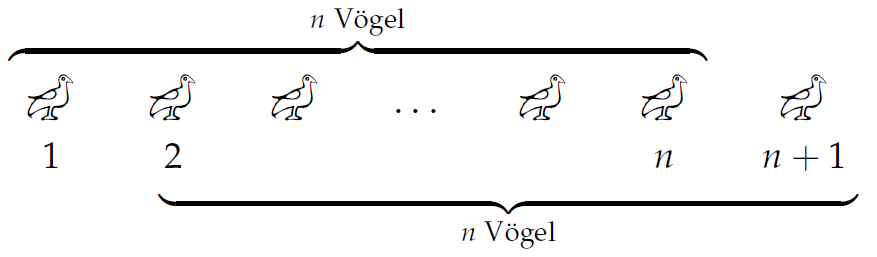
\includegraphics[scale=0.4]{induktion_voegel}
			\centering
		\end{figure}
	
		\only<5|handout:4>{
			Die Vögel $1, 2, ..., n$ bilden eine Menge mit genau $n$ Vögeln. Also haben sie nach IV alle die gleiche Farbe.\\ 
			Die Vögel $2, 3, ..., n + 1$ bilden auch eine Menge mit genau $n$ Vögeln. Also haben nach IV auch diese alle die gleiche Farbe.\\
			Damit haben auch die Vögel $1$ und $n + 1$ die gleiche Farbe, also haben alle Vögel die gleiche Farbe. $\qed$
		}
	\end{block}
	}
\end{frame}

\begin{frame}[t]{Vogelfarben: Auflösung}
	\begin{block}{Was geht schief?}
		\begin{figure}
			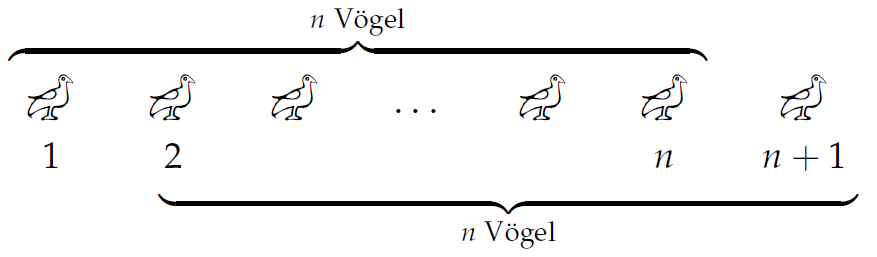
\includegraphics[scale=0.4]{induktion_voegel}
			\centering
		\end{figure}
		\pause
		Hübsches Bild. Scheint sauber. Ist bloß für $n=2$ völlig kaputt, die beiden Teilmengen \textbf{überlappen sich} dann nämlich \textbf{nicht}. \\
		\impl Wir können nicht sagen, dass der erste und letzte Vogel immer die gleiche Farbe haben. (Und wenn schon zwei Vögel nicht immer die gleiche Farbe haben, dann drei etc. auch nicht.) \\
		\impl Ganze Induktion \textbf{kaputt}. \frownie
	\end{block}	
	%Das Bild ist zwar außerordentlich hübsch, suggeriert aber leider etwas, was nicht immer stimmt: Für $n = 2$ überlappen sich die Teilmengen „ohne den ersten“ und „ohne den letzten“ Vogel nicht. Es ist also nicht erzwungen, dass beide Vögel die gleiche Farbe haben. (Und das macht „alles weitere“ auch kaputt: Wenn nicht immer 2 Vögel die gleiche Farbe haben, dann auch nicht immer 3 Vögel, usw.)
\end{frame}

% Induktion Übung

\begin{frame}{Und jetzt ihr}
    Betrachten Sie die Abbildung $f: \N_0 \to \N_0$, die wie folgt festgelegt ist:
    \begin{align*}
        f(0) = 0&&\forall n \in \N_0: f(n+1) = 2f(n) + n + 5
    \end{align*}
% 	Behauptung: \[\forall n \in \N_+ : \sum_{k=0}^{n}{\frac{1}{2^k}} = 2 \* \tuple{1 - \frac{1}{2^{n+1}}}\]
    Beweisen Sie durch vollständige Induktion, dass für jedes $n \in \N_0$ gilt:
    \[f(n) = 6(2^n - 1) - n\]
	\pause
	\begin{block}{Induktionsanfang}
		$n = 0$: $f(0)=0 = 6 \cdot 0 - 0 = 6 \cdot (2^0 - 1) - 0 $. \; \textbf{\checked}
	\end{block}
	\pause
	\begin{block}{Induktionsvoraussetzung}
		Für ein $n \in \N_0$ gelte: $f(n) = 6(2^n - 1) - n$.
	\end{block}
\end{frame}

\begin{frame}[t]
	\begin{block}{Induktionsvoraussetzung}
		Für ein $n \in \N_0$ gelte: $f(n) = 6(2^n - 1) - n$.
	\end{block}
	\uncover<+->{}
	\begin{block}{Induktionsschritt}
		Zeige die Aussage für $n+1$:\\
		\begin{align*}
			f(n+1)
				&= \uncover<+->{2f(n)+n+5}\\
				\uncover<+->{&\stackrel{\text{IV}}{=} 2(6(2^n-1)-n)+n+5\\}
				\uncover<+->{
				&= 6(2^{n+1}-2)-2n+n+5\\}
				\uncover<+->{
				&= 6(2^{n+1}-1)-6-n-1+6\\}
				\uncover<+->{
				&= 6(2^{n+1}-1)-(n+1) \qed}
		\end{align*}
	\end{block}
\end{frame}

\begin{frame}{Und jetzt ihr}
	Behauptung: \[\forall n \in \N_+ : \sum_{k=0}^{n}{\frac{1}{2^k}} = 2 \* \tuple{1 - \frac{1}{2^{n+1}}}\]
	\pause
	\begin{block}{Induktionsanfang}
		$n = 1$: $\sum_{k=0}^{1}{\frac{1}{2^k}} = \frac{3}{2} = 2 \* \frac{3}{4}$. \; \textbf{\checked}
	\end{block}
	\pause
	\begin{block}{Induktionsvoraussetzung}
		Für ein $n \in \N_0$ gelte: $\sum_{k=0}^{n}{\frac{1}{2^k}} = 2 \* \tuple{1 - \frac{1}{2^{n+1}}}$.
	\end{block}
\end{frame}

\begin{frame}[t]
	\uncover<+->{}
	\begin{block}{Induktionsschritt}
		Zeige die Aussage für $n+1$:\\
		\begin{align*}
			\sum_{k=0}^{n+1}{\frac{1}{2^k}}
				&= \uncover<+->{\underbrace{\sum_{k=0}^{n}{\frac{1}{2^k}}}_{\stackrel{\text{IV}}{=} 2 \* \tuple{1 - \frac{1}{2^{n+1}}}} + \frac{1}{2^{n+1}}}\\
				\uncover<+->{&= 2 \* \left(1 - \frac{1}{2^{n+1}}\right) + \frac{1}{2^{n+1}}\\
				&= 2 \* \left(1 - \frac{2}{2^{n+2}} + \frac{1}{2^{n+2}}\right)\\
				&= 2 \* \left(1 - \frac{1}{2^{(n+1)+1}}\right). \qed}
		\end{align*}
	\end{block}
\end{frame}

% Induktion Wörter Länge
% \begin{frame}{Und jetzt mit Wörtern}
% 	\begin{block}{Behauptung}
% 		Seien $A, B$ zwei beliebige Alphabete. Definiere die Funktion $f \from A^* \functionto A^*$,
% 		\begin{align*}
% 			f(\eps) &:= \eps \\
% 			\text{Für } w \in A^*, \mu \in A: \quad f(\mu \* w) &:= 
% 			\begin{cases}
% 				\mu \* f(w), &\mu \in B \\
% 				f(w), &\text{sonst}
% 			\end{cases}\\
% 		\end{align*}
	
% 	Dann gilt $\forall w \in A^*: \size{f(w)} \le \size w$.
% 	\end{block}
% \end{frame}

% \begin{frame}{Und jetzt mit Wörtern}
% 	Induktion über die Wortlänge ($n = \size w$):\\[0.5em]
% 	\pause
% 	\begin{block}{Induktionsanfang}
% 		$n = 0$: Nur das leere Wort hat Länge 0. Also $w = \eps$.\\
% 		$f(\eps) = \eps \impl \size{f(w)} = \size w = 0$. \; \textbf{\checked}
% 	\end{block}
% 	\pause
% 	\begin{block}{Induktionsvoraussetzung}
% 		Für \textbf{ein} $n \in \N_0$ gelte: Für alle Wörter der Länge $n$ über $A$ (also $w \in A^n$) ist $\size{f(w)} \le \size w$.
% 	\end{block}
% \end{frame}

% \begin{frame}{Und jetzt mit Wörtern}
% 	\begin{block}{Induktionsschritt}
% 		Zeige die Aussage für $n+1$:\\
% 		Sei $w \in A^{n+1}$ ein Wort der Länge $n+1$.\\
% 		\pause
% 		Dann teilen wir es auf in $w = \mu \* v$, wobei $\mu \in A$ und $v \in A^n$.\\
% 		Nach IV gilt: $\size{f(v)} \le \size v$.\\
% 		\pause
% 		\smallskip
% 		\textbf{Fall 1}: \\
% 			\quad $\mu \in B$: $f(w) = \mu \* f(v)$ \\
% 			\quad \impl $\size{f(w)} = 1 + \size{f(v)} \le 1 + \size v = 1+n = \size w$.\\
% 		\pause
% 		\smallskip
% 		\textbf{Fall 2}: \\
% 			\quad $\mu \notin B$: $f(w) = f(v)$ \\
% 			\quad \impl $\size{f(w)} = \size{f(v)} \le \size v = n \le n+1 = \size w$.\\
% 		\pause
% 		\smallskip
% 		Also gilt: $\size{f(w)} \le \size w. \qed$
% 	\end{block}
% \end{frame}

\appendix
\beginbackup

\section{Zusammenfassung und Ausblick}

\begin{frame}
	\begin{block}{Was ihr nun wissen solltet}
		\begin{itemize}
			\item Wie vollständige Induktion geht
			\item Aussagenlogik: Syntax und Semantik
			\item Wie man wahre Aussagen konstruiert \qquad (\#NoFakeNews!)
		\end{itemize}
	\end{block}

	\begin{block}{Was nächstes Mal kommt}
		\begin{itemize}
			\item Induktion
			\item Formale Sprachen
			\item Aus \word2 mach \word{10}: Übersetzungen
		\end{itemize}
	\end{block}
\end{frame}


\only<handout:0>{\slideThanks}

\xkcdframe{589}{Danke für eure Aufmerksamkeit! \smiley}{2}

\only<beamer:0>{\slideThanks}

\backupend

\end{document}
